% answers.tex —— 2014 年全国Ⅰ卷（文科） · 参考答案与详细解析片段
% 由 tools/generate_projects.py 依来源总账自 2014/2014_数学真题_全国1文_试题.md + 2014/2014_数学真题_全国1文_解析正文.md + 2014/2014_数学真题_全国1文_答案要点.md 生成，勿手改（改源 MD 后重跑）


\begin{gktip}
固定源 PDF 是印刷页码 901–902 的两页题面，不附答案或解析。以下各题均依据题面独立复算，\textbf{非官方标准答案}；第 8、9、16、18、19、22 题图形在 LaTeX 工程中以 TikZ/PGFPlots 矢量源重绘。第 18 题的题面图是待作答的空白频率分布直方图框，重绘时不预先填入柱条。
\end{gktip}

\gkpart{一、选择题}

\begin{answer}
\gksolhead{1}{}

\textbf{题目}：

已知集合 $M=\{x\mid -1<x<3\}$，$N=\{x\mid -2<x<1\}$，则 $M\cap N=$\mbox{（　　）}

（A）$(-2,1)$　　（B）$(-1,1)$　　（C）$(1,3)$　　（D）$(-2,3)$

\Needspace{4\baselineskip}
\textbf{解析}

两开区间的公共部分为 $(-1,1)$，故选 B。

\gkanswer{答案：B}

\end{answer}
\begin{answer}
\gksolhead{2}{}

\textbf{题目}：

若 $\tan\alpha>0$，则\mbox{（　　）}

（A）$\sin2\alpha>0$　　（B）$\cos\alpha>0$　　（C）$\sin\alpha>0$　　（D）$\cos2\alpha>0$

\Needspace{4\baselineskip}
\textbf{解析}

$\tan\alpha>0$ 表示 $\sin\alpha,\cos\alpha$ 同号，故 $\sin2\alpha=2\sin\alpha\cos\alpha>0$；其余三式的符号均不能由题设唯一确定，选 A。

\gkanswer{答案：A}

\end{answer}
\begin{answer}
\gksolhead{3}{}

\textbf{题目}：

设 $z=\dfrac1{1+i}+i$，则 $|z|=$\mbox{（　　）}

（A）$\dfrac12$　　（B）$\dfrac{\sqrt2}{2}$　　（C）$\dfrac{\sqrt3}{2}$　　（D）$2$

\Needspace{4\baselineskip}
\textbf{解析}

\nopagebreak[4]
\[
z=\frac{1-i}{2}+i=\frac{1+i}{2},\qquad |z|=\frac{\sqrt2}{2},
\]

故选 B。

\gkanswer{答案：B}

\end{answer}
\begin{answer}
\gksolhead{4}{}

\textbf{题目}：

已知双曲线 $\dfrac{x^2}{a^2}-\dfrac{y^2}{3}=1\ (a>0)$ 的离心率为 $2$，则 $a=$\mbox{（　　）}

（A）$2$　　（B）$\dfrac{\sqrt6}{2}$　　（C）$\dfrac{\sqrt5}{2}$　　（D）$1$

\Needspace{4\baselineskip}
\textbf{解析}

由 $e^2=1+3/a^2=4$ 得 $a^2=1$。又 $a>0$，故 $a=1$；按选项为 A。

\gkanswer{答案：A}

\end{answer}
\begin{answer}
\gksolhead{5}{}

\textbf{题目}：

设函数 $f(x),g(x)$ 的定义域都为 $\mathbb R$，且 $f(x)$ 是奇函数，$g(x)$ 是偶函数，则下列结论正确的是\mbox{（　　）}

（A）$f(x)|g(x)|$ 是奇函数　　（B）$|f(x)|g(x)$ 是奇函数

（C）$f(x)g(x)$ 是偶函数　　（D）$|f(x)g(x)|$ 是奇函数

\Needspace{4\baselineskip}
\textbf{解析}

$|g(x)|$ 为偶函数，奇函数 $f(x)$ 与它的乘积仍为奇函数，故 A 正确。$|f(x)|g(x)$、$f(x)g(x)$ 与 $|f(x)g(x)|$ 均为偶函数。

\gkanswer{答案：A}

\end{answer}
\begin{answer}
\gksolhead{6}{}

\textbf{题目}：

设 $D,E,F$ 分别为 $\triangle ABC$ 的三边 $BC,CA,AB$ 的中点，则 $\overrightarrow{EB}+\overrightarrow{FC}=$\mbox{（　　）}

（A）$\overrightarrow{BC}$　　（B）$\dfrac12\overrightarrow{AD}$　　（C）$\overrightarrow{AD}$　　（D）$\dfrac12\overrightarrow{BC}$

\Needspace{4\baselineskip}
\textbf{解析}

\Needspace{5\baselineskip}
取 $A$ 为原点，记 $\overrightarrow{AB}=\boldsymbol b$、$\overrightarrow{AC}=\boldsymbol c$。则

\nopagebreak[4]
\[
\overrightarrow{EB}+\overrightarrow{FC}
=\left(\boldsymbol b-\frac{\boldsymbol c}{2}\right)+\left(\boldsymbol c-\frac{\boldsymbol b}{2}\right)
=\frac{\boldsymbol b+\boldsymbol c}{2}=\frac12\overrightarrow{AD}.
\]

故选 B。

\gkanswer{答案：B}

\end{answer}
\begin{answer}
\gksolhead{7}{}

\textbf{题目}：

在函数① $y=\cos|2x|$，② $y=|\cos x|$，③ $y=\cos\left(2x+\dfrac\pi6\right)$，④ $y=\tan\left(2x-\dfrac\pi4\right)$ 中，最小正周期为 $\pi$ 的所有函数为\mbox{（　　）}

（A）②④　　（B）①③④　　（C）①②③　　（D）①③

\Needspace{4\baselineskip}
\textbf{解析}

$\cos|2x|=\cos2x$，最小正周期为 $\pi$；$|\cos x|$ 的最小正周期也为 $\pi$；平移不改变 $\cos2x$ 的周期；$\tan(2x-\pi/4)$ 的最小正周期为 $\pi/2$。故为①②③，选 C。

\gkanswer{答案：C}

\end{answer}
\begin{answer}
\gksolhead{8}{}

\textbf{题目}：

如图，网格纸的各小格都是正方形，粗实线画出的是一个几何体的三视图，则这个几何体是\mbox{（　　）}
\nopagebreak[4]
\begin{center}% 2014 全国卷Ⅰ文科第 8 题：方格纸上的三视图。
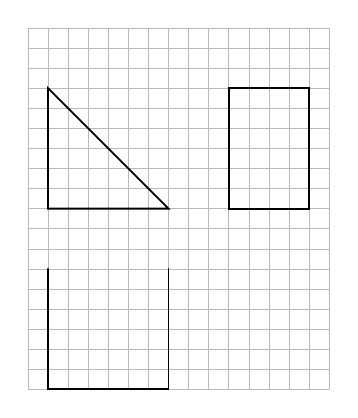
\begin{tikzpicture}[x=2.55mm,y=2.55mm,line cap=round]
  % 细灰色方格；粗实线是题面给出的三个投影。
  \draw[step=1,gray!55,line width=.18pt] (0,0) grid (15,18);
  \draw[line width=.65pt] (1,15)--(1,9)--(7,9)--cycle;
  \draw[line width=.65pt] (10,15)--(14,15)--(14,9)--(10,9)--cycle;
  \draw[line width=.65pt] (1,6)--(1,0)--(7,0)--(7,6);
\end{tikzpicture}
\end{center}
\nopagebreak[4]
（A）三棱锥　　（B）三棱柱　　（C）四棱锥　　（D）四棱柱

\Needspace{4\baselineskip}
\textbf{解析}

三个投影中，三角形轮廓与两个矩形投影相对应，空间几何体为三棱柱，选 B。

\gkanswer{答案：B}

\end{answer}
\begin{answer}
\gksolhead{9}{}

\textbf{题目}：

执行如图的程序框图，若输入的 $a,b,k$ 分别为 $1,2,3$，则输出的 $M=$\mbox{（　　）}
\nopagebreak[4]
\begin{center}% 2014 全国卷Ⅰ文科第 9 题：迭代计算程序框图。
\begin{tikzpicture}[font=\footnotesize,>=Stealth,node distance=4mm,line width=.4pt,
  box/.style={draw,minimum height=1.65em,minimum width=6.4em,inner xsep=5pt},
  term/.style={draw,rounded corners=6pt,minimum height=1.65em,inner xsep=8pt},
  io/.style={draw,trapezium,trapezium left angle=70,trapezium right angle=110,
             minimum height=1.65em,inner xsep=4pt},
  dec/.style={draw,diamond,aspect=2.25,inner sep=1.6pt}]
  \node[term] (start) {开始};
  \node[io,below=of start] (input) {输入 $a,b,k$};
  \node[box,below=of input] (init) {$n=1$};
  \node[dec,below=7mm of init] (cond) {$n\leqslant k$};
  \node[box,below=8mm of cond] (calc) {$M=a+\dfrac1b$};
  \node[box,below=of calc] (seta) {$a=b$};
  \node[box,below=of seta] (setb) {$b=M$};
  \node[box,below=of setb] (inc) {$n=n+1$};
  \node[io,left=23mm of calc] (output) {输出 $M$};
  \node[term,below=of output] (end) {结束};
  \draw[->] (start)--(input)--(init)--(cond);
  \draw[->] (cond)--node[right] {是}(calc)--(seta)--(setb)--(inc);
  \draw[->] (inc.east)-| ([xshift=19mm]cond.east) |- (cond.north);
  \draw[->] (cond.west)-|node[pos=.17,above] {否}(output.north);
  \draw[->] (output)--(end);
\end{tikzpicture}
\end{center}
\nopagebreak[4]
（A）$\dfrac{20}{3}$　　（B）$\dfrac72$　　（C）$\dfrac{16}{5}$　　（D）$\dfrac{15}{8}$

\Needspace{4\baselineskip}
\textbf{解析}

\Needspace{5\baselineskip}
按框图迭代：

\nopagebreak[4]
\[
(a,b)=(1,2)\to\left(2,\frac32\right)\to\left(\frac32,\frac83\right).
\]

\Needspace{5\baselineskip}
第 $3$ 次循环计算

\nopagebreak[4]
\[
M=\frac32+\frac1{8/3}=\frac{15}{8}.
\]

随后 $n=4>k$，输出该值，选 D。

\gkanswer{答案：D}

\end{answer}
\begin{answer}
\gksolhead{10}{}

\textbf{题目}：

已知抛物线 $C:y^2=x$ 的焦点为 $F$，$A(x_0,y_0)$ 是 $C$ 上一点，$|AF|=\dfrac54x_0$，则 $x_0=$\mbox{（　　）}

（A）$4$　　（B）$2$　　（C）$1$　　（D）$8$

\Needspace{4\baselineskip}
\textbf{解析}

\Needspace{5\baselineskip}
抛物线 $y^2=x$ 的焦点为 $(1/4,0)$。对抛物线上点 $A(x_0,y_0)$，有 $|AF|=x_0+1/4$。由题设

\nopagebreak[4]
\[
x_0+\frac14=\frac54x_0
\]

得 $x_0=1$，选 C。

\gkanswer{答案：C}

\end{answer}
\begin{answer}
\gksolhead{11}{}

\textbf{题目}：

\Needspace{5\baselineskip}
设 $x,y$ 满足约束条件

\nopagebreak[4]
\[
\begin{cases}
x+y\geqslant a,\\
x-y\leqslant-1,
\end{cases}
\]

且 $z=x+ay$ 的最小值为 $7$，则 $a=$\mbox{（　　）}

（A）$-5$　　（B）$3$　　（C）$-5$ 或 $3$　　（D）$5$ 或 $-3$

\Needspace{4\baselineskip}
\textbf{解析}

\Needspace{5\baselineskip}
可行域为 $y\geqslant\max\{a-x,x+1\}$。要使 $x+ay$ 有最小值，须 $a\geqslant0$，其最小值在两边界交点

\nopagebreak[4]
\[
\left(\frac{a-1}{2},\frac{a+1}{2}\right)
\]

\Needspace{5\baselineskip}
处取得。因此

\nopagebreak[4]
\[
\frac{a-1}{2}+a\frac{a+1}{2}=7,
\]

即 $a^2+2a-15=0$。结合 $a\geqslant0$，得 $a=3$，选 B。

\gkanswer{答案：B}

\end{answer}
\begin{answer}
\gksolhead{12}{}

\textbf{题目}：

已知函数 $f(x)=ax^3-3x^2+1$，若 $f(x)$ 存在唯一的零点 $x_0$，且 $x_0>0$，则 $a$ 的取值范围为\mbox{（　　）}

（A）$(-\infty,-2)$　　（B）$(1,+\infty)$　　（C）$(2,+\infty)$　　（D）$(-\infty,-1)$

\Needspace{4\baselineskip}
\textbf{解析}

\nopagebreak[4]
\[
f'(x)=3x(ax-2).
\]

当 $a<0$ 时，若 $a<-2$，极小值 $f(2/a)=1-4/a^2>0$，图象只在正半轴与 $x$ 轴相交一次。$a=-2$ 时还出现负根的重根；$-2<a<0$ 时有三个零点。$a>0$ 时不可能恰有一个正零点。故 $a\in(-\infty,-2)$，选 A。

\gkanswer{答案：A}

\end{answer}
\gkpart{二、填空题}

\begin{answer}
\gksolhead{13}{}

\textbf{题目}：

将 $2$ 本不同的数学书和 $1$ 本语文书在书架上随机排成一行，则 $2$ 本数学书相邻的概率为\gkblank{}。

\Needspace{4\baselineskip}
\textbf{解析}

三本书任排有 $3!=6$ 种。将两本数学书视为一组，则相邻排法有 $2\times2=4$ 种，概率为 $4/6=2/3$。

\gkanswer{答案：$\dfrac23$}

\end{answer}
\begin{answer}
\gksolhead{14}{}

\textbf{题目}：

甲、乙、丙三位同学被问到是否去过 $A,B,C$ 三个城市时，甲说：我去过的城市比乙多，但没去过 $B$ 城市；乙说：我没去过 $C$ 城市；丙说：我们三人去过同一个城市。由此可判断乙去过的城市为\gkblank{}。

\Needspace{4\baselineskip}
\textbf{解析}

三人共同去过的城市不能是 $B$（甲未去），也不能是 $C$（乙未去），故必为 $A$。若乙还去过 $B$，乙已去两城，而甲未去 $B$ 至多去 $A,C$ 两城，不能满足甲去得更多。故乙只去过 $A$ 城市。

\gkanswer{答案：$A$ 城市}

\end{answer}
\begin{answer}
\gksolhead{15}{}

\textbf{题目}：

\Needspace{5\baselineskip}
设函数

\nopagebreak[4]
\[
f(x)=\begin{cases}
e^{x-1},&x<1,\\
x^{\frac13},&x\geqslant1,
\end{cases}
\]

则使得 $f(x)\leqslant2$ 成立的 $x$ 的取值范围是\gkblank{}。

\Needspace{4\baselineskip}
\textbf{解析}

当 $x<1$，$e^{x-1}<1<2$；当 $x\geqslant1$，不等式为 $x^{1/3}\leqslant2$，即 $x\leqslant8$。合并得 $(-\infty,8]$。

\gkanswer{答案：$(-\infty,8]$}

\end{answer}
\begin{answer}
\gksolhead{16}{}

\textbf{题目}：

如图，为测量山高 $MN$，选择 $A$ 和另一座山的山顶 $C$ 为测量观测点。从 $A$ 点测得 $M$ 点的仰角 $\angle MAN=60^\circ$，$C$ 点的仰角 $\angle CAB=45^\circ$ 以及 $\angle MAC=75^\circ$；从 $C$ 点测得 $\angle MCA=60^\circ$。已知山高 $BC=100\ \mathrm m$，则山高 $MN=$\gkblank{} $\mathrm m$。
\nopagebreak[4]
\begin{center}% 2014 全国卷Ⅰ文科第 16 题：测量山高的观测示意图。
\begin{tikzpicture}[font=\footnotesize,line width=.45pt,line cap=round,line join=round]
  \coordinate (A) at (0,0);
  \coordinate (B) at (4.5,0);
  \coordinate (C) at (4.5,2.25);
  \coordinate (N) at (-1.9,.82);
  \coordinate (M) at (-1.9,5.05);
  \draw (M)--(N);
  \draw (B)--(C);
  \draw (A)--(B);
  \draw (A)--(M) (A)--(C) (C)--(M);
  \draw[dashed] (N)--(B);
  \draw[dashed] (N)--(A);
  \node[above] at (M) {$M$};
  \node[left] at (N) {$N$};
  \node[below] at (A) {$A$};
  \node[below] at (B) {$B$};
  \node[right] at (C) {$C$};
\end{tikzpicture}
\end{center}
\nopagebreak[4]
\Needspace{4\baselineskip}
\textbf{解析}

\Needspace{5\baselineskip}
取 $A$ 所在水平线为基准。由 $\angle CAB=45^\circ$、$BC=100\ \mathrm m$，得 $A$ 与 $B$ 的水平距离为 $100\ \mathrm m$。在 $\triangle AMC$ 中，

\nopagebreak[4]
\[
\angle MAC=75^\circ,\qquad \angle MCA=60^\circ,
\]

\Needspace{5\baselineskip}
所以 $\angle AMC=45^\circ$。由正弦定理

\nopagebreak[4]
\[
\frac{AM}{\sin60^\circ}=\frac{AC}{\sin45^\circ}
=\frac{100\sqrt2}{\sin45^\circ}=200,
\]

\Needspace{5\baselineskip}
故 $AM=100\sqrt3$。又 $\angle MAN=60^\circ$，山高

\nopagebreak[4]
\[
MN=AM\sin60^\circ=150\ \mathrm m.
\]

\gkanswer{答案：$150$}

\end{answer}
\gkpart{三、解答题}

\begin{answer}
\gksolhead{17}{}

\textbf{题目}：

已知 $\{a_n\}$ 是递增的等差数列，$a_2,a_4$ 是方程 $x^2-5x+6=0$ 的根。

(1) 求 $\{a_n\}$ 的通项公式；

(2) 求数列 $\left\{\dfrac{a_n}{2^n}\right\}$ 的前 $n$ 项和。

\Needspace{4\baselineskip}
\textbf{解析}

\gksubpart{(1) 求通项}

\Needspace{5\baselineskip}
方程两根为 $2,3$。数列递增，故 $a_2=2,a_4=3$，从而公差 $d=1/2$，首项 $a_1=3/2$。所以

\nopagebreak[4]
\[
a_n=\frac{n+2}{2}.
\]

\gksubpart{(2) 求前 $n$ 项和}

\nopagebreak[4]
\[
\frac{a_k}{2^k}=\frac{k+2}{2^{k+1}}.
\]

\Needspace{5\baselineskip}
用 $\sum_{k=1}^n k/2^k=2-(n+2)/2^n$ 和等比数列求和，得

\nopagebreak[4]
\[
\sum_{k=1}^n\frac{a_k}{2^k}
=\frac12\sum_{k=1}^n\frac{k+2}{2^k}
=2-\frac{n+4}{2^{n+1}}.
\]

\gkanswer{答案（1）：$a_n=\dfrac{n+2}{2}$}

\gkanswer{答案（2）：$2-\dfrac{n+4}{2^{n+1}}$}

\end{answer}
\begin{answer}
\gksolhead{18}{}

\textbf{题目}：

从某企业生产的某种产品中抽取 $100$ 件，测量这些产品的一项质量指标值，由测量结果得如下频数分布表：

\begin{center}
\begin{tabular}{lrrrrr}
\toprule
质量指标值分组 & $[75,85)$ & $[85,95)$ & $[95,105)$ & $[105,115)$ & $[115,125)$ \\
\midrule
频数 & $6$ & $26$ & $38$ & $22$ & $8$ \\
\bottomrule
\end{tabular}
\end{center}

(1) 作出这些数据的频率分布直方图；
\nopagebreak[4]
\begin{center}% 2014 全国卷Ⅰ文科第 18 题：频率分布直方图的待作答空白框。
% 有意不画任何柱条；原题要求考生据频数表自行作图。
\begin{tikzpicture}[font=\scriptsize,>=Stealth,line cap=round]
  \draw[gray!58,line width=.22pt] (.6,0) grid[xstep=1,ystep=.5] (5.6,10);
  \draw[->,line width=.45pt] (-.62,0)--(6.32,0) node[right] {质量指标值};
  \draw[->,line width=.45pt] (0,-.18)--(0,10.72) node[above left,align=center] {频率\\组距};
  % 原点后的断轴锯齿。
  \draw[line width=.4pt] (.14,.10)--(.22,-.10)--(.30,.10)--(.38,-.10)--(.46,.10);
  \foreach \x/\lab in {.6/75,1.6/85,2.6/95,3.6/105,4.6/115,5.6/125}
    \node[below=2pt] at (\x,0) {\lab};
  \node[below=2pt] at (-.38,0) {0};
  \foreach \k in {1,...,20}
    \pgfmathsetmacro\v{\k/500}
    \node[left=2pt] at (0,\k/2) {\pgfmathprintnumber[fixed,fixed zerofill,precision=3]{\v}};
\end{tikzpicture}
\end{center}
\nopagebreak[4]
(2) 估计这种产品质量指标值的平均数及方差（同一组中的数据用该组区间的中点值作代表）；

(3) 根据以上抽样调查数据，能否认为该企业生产的这种产品符合“质量指标值不低于 $95$ 的产品至少要占全部产品的 $80\%$”的规定？

\par\medskip

*以下续自固定源 PDF 第 2 页（印刷页 902）。*

\Needspace{4\baselineskip}
\textbf{解析}

\gksubpart{(1) 作频率分布直方图}

\Needspace{5\baselineskip}
各组频率为 $0.06,0.26,0.38,0.22,0.08$，组距均为 $10$，故柱高（频率/组距）依次为

\nopagebreak[4]
\[
0.006,\quad0.026,\quad0.038,\quad0.022,\quad0.008.
\]

这些数是对作图小问的计算结果；题面原图保持为空白坐标框，不在题面中预填柱条。

\gksubpart{(2) 估计平均数及方差}

\Needspace{5\baselineskip}
以 $80,90,100,110,120$ 为各组代表值，

\nopagebreak[4]
\[
\bar x=80\times0.06+90\times0.26+100\times0.38+110\times0.22+120\times0.08=100.
\]

\Needspace{5\baselineskip}
方差估计为

\nopagebreak[4]
\[
20^2\times0.06+10^2\times0.26+10^2\times0.22+20^2\times0.08=104.
\]

\gksubpart{(3) 判断是否符合规定}

\Needspace{5\baselineskip}
质量指标值不低于 $95$ 的样本频率为

\nopagebreak[4]
\[
\frac{38+22+8}{100}=0.68<0.80.
\]

因此不能认为该企业生产的产品符合该规定。

\gkanswer{答案（1）：各组频率/组距依次为 $0.006,0.026,0.038,0.022,0.008$；在题给空白直方图的五个组距内分别作对应高度的柱形。}

\gkanswer{答案（2）：平均数估计为 $100$，方差估计为 $104$。}

\gkanswer{答案（3）：不能认为符合；样本中不低于 $95$ 的频率为 $0.68<0.80$。}

\end{answer}
\begin{answer}
\gksolhead{19}{}

\textbf{题目}：

如图，三棱柱 $ABC-A_1B_1C_1$ 中，侧面 $BB_1C_1C$ 为菱形，$B_1C$ 的中点为 $O$，且 $AO\perp$ 平面 $BB_1C_1C$。
\nopagebreak[4]
\begin{center}% 2014 全国卷Ⅰ文科第 19 题：三棱柱及侧面内的中点 O。
\begin{tikzpicture}[font=\footnotesize,line width=.45pt,line cap=round,line join=round]
  \coordinate (B) at (0,0);
  \coordinate (C) at (1.55,.82);
  \coordinate (B1) at (3.20,0);
  \coordinate (C1) at (4.70,.82);
  \coordinate (A) at (1.72,2.72);
  \coordinate (A1) at (4.92,2.72);
  \coordinate (O) at ($(B1)!0.5!(C)$);
  \draw (B)--(A)--(B1)--(A1)--(C1)--(B1);
  \draw (A)--(A1) (B1)--(C1) (B)--(B1);
  \draw[dashed] (B)--(C)--(A) (C)--(C1) (C)--(B1) (A)--(O);
  \node[below left] at (B) {$B$};
  \node[left] at (C) {$C$};
  \node[below] at (B1) {$B_1$};
  \node[right] at (C1) {$C_1$};
  \node[above] at (A) {$A$};
  \node[above] at (A1) {$A_1$};
  \node[below left] at (O) {$O$};
\end{tikzpicture}
\end{center}
\nopagebreak[4]
(1) 证明：$B_1C\perp AB$；

(2) 若 $AC\perp AB_1$，$\angle CBB_1=60^\circ$，$BC=1$，求三棱柱 $ABC-A_1B_1C_1$ 的高。

\Needspace{4\baselineskip}
\textbf{解析}

\gksubpart{(1) 证明垂直}

\Needspace{5\baselineskip}
设 $O$ 为原点，取侧面 $BB_1C_1C$ 为基面。菱形对角线互相平分，故

\nopagebreak[4]
\[
\overrightarrow{OB}+\overrightarrow{OB_1}=\overrightarrow{OC}+\overrightarrow{OC_1}=\boldsymbol0,
\]

\Needspace{5\baselineskip}
且 $O$ 是 $B_1C$ 的中点。由 $AO\perp$ 该平面，$\overrightarrow{AO}$ 垂直于平面内任意向量。于是

\nopagebreak[4]
\[
\overrightarrow{AB}\cdot\overrightarrow{B_1C}
=\left(\overrightarrow{AO}+\overrightarrow{OB}\right)\cdot
\left(\overrightarrow{OC}-\overrightarrow{OB_1}\right)=0,
\]

所以 $B_1C\perp AB$。

\gksubpart{(2) 求高}

\Needspace{5\baselineskip}
令 $BC=BB_1=1$，在侧面内取

\nopagebreak[4]
\[
B=(0,0,0),\ C=(1,0,0),\ B_1=\left(\frac12,\frac{\sqrt3}{2},0\right).
\]

\Needspace{5\baselineskip}
则 $O=(3/4,\sqrt3/4,0)$，可设 $A=(3/4,\sqrt3/4,h)$。由棱柱平移关系，

\nopagebreak[4]
\[
\overrightarrow{AC}=\left(\frac14,-\frac{\sqrt3}{4},-h\right),\quad
\overrightarrow{AB_1}=\left(-\frac14,\frac{\sqrt3}{4},-h\right).
\]

条件 $AC\perp AB_1$ 给出 $h^2-1/4=0$。高为正，故 $h=1/2$。

\gkanswer{答案（1）：见解析版}

\gkanswer{答案（2）：$\dfrac12$}

\end{answer}
\begin{answer}
\gksolhead{20}{}

\textbf{题目}：

已知点 $P(2,2)$，圆 $C:x^2+y^2-8y=0$，过点 $P$ 的动直线 $l$ 与圆 $C$ 交于 $A,B$ 两点，线段 $AB$ 的中点为 $M$，$O$ 为坐标原点。

(1) 求 $M$ 的轨迹方程；

(2) 当 $|OP|=|OM|$ 时，求 $l$ 的方程及 $\triangle POM$ 的面积。

\Needspace{4\baselineskip}
\textbf{解析}

\gksubpart{(1) 求轨迹方程}

\Needspace{5\baselineskip}
圆心为 $C(0,4)$。弦中点 $M(x,y)$ 满足 $CM\perp PM$，故

\nopagebreak[4]
\[
(x,y-4)\cdot(x-2,y-2)=0,
\]

\Needspace{5\baselineskip}
化简得

\nopagebreak[4]
\[
x^2+y^2-2x-6y+8=0.
\]

\gksubpart{(2) 求直线和面积}

\Needspace{5\baselineskip}
又 $|OM|=|OP|=2\sqrt2$，故联立上式与 $x^2+y^2=8$，得

\nopagebreak[4]
\[
M=(-2,2)\quad\text{\text{或}}\quad M=\left(\frac{14}{5},\frac25\right).
\]

相应直线 $PM$ 分别为 $y=2$、$2x+y-6=0$。用行列式求面积，分别为 $4$、$12/5$。

\gkanswer{答案（1）：$x^2+y^2-2x-6y+8=0$。}

\gkanswer{答案（2）：$l:y=2$，此时面积为 $4$；或 $l:2x+y-6=0$，此时面积为 $\dfrac{12}{5}$。}

\end{answer}
\begin{answer}
\gksolhead{21}{}

\textbf{题目}：

设函数 $f(x)=a\ln x+\dfrac{1-a}{2}x^2-bx\ (a\ne1)$，曲线 $y=f(x)$ 在点 $(1,f(1))$ 处的切线斜率为 $0$。

(1) 求 $b$；

(2) 若存在 $x_0\geqslant1$ 使得 $f(x_0)<\dfrac{a}{a-1}$，求 $a$ 的取值范围。

\Needspace{4\baselineskip}
\textbf{解析}

\gksubpart{(1) 求 $b$}

\nopagebreak[4]
\[
f'(x)=\frac ax+(1-a)x-b,
\]

由 $f'(1)=0$ 得 $b=1$。

\gksubpart{(2) 求 $a$ 的范围}

\Needspace{5\baselineskip}
代入 $b=1$，有

\nopagebreak[4]
\[
f'(x)=\frac{(x-1)((1-a)x-a)}{x}.
\]

\Needspace{5\baselineskip}
当 $a>1$ 时，$f(x)\to-\infty\ (x\to+\infty)$，条件成立。当 $1/2<a<1$ 时，$x=a/(1-a)$ 为 $[1,+\infty)$ 上的极小点，代入可知极小值不小于 $a/(a-1)$。当 $a\leqslant1/2$ 时，最小值为 $f(1)=-(a+1)/2$，条件化为

\nopagebreak[4]
\[
-\frac{a+1}{2}<\frac a{a-1}
\iff a^2+2a-1<0.
\]

\Needspace{5\baselineskip}
综合并注意 $a\ne1$，得

\nopagebreak[4]
\[
a\in(-1-\sqrt2,\sqrt2-1)\cup(1,+\infty).
\]

\gkanswer{答案（1）：$b=1$。}

\gkanswer{答案（2）：$(-1-\sqrt2,\sqrt2-1)\cup(1,+\infty)$。}

\end{answer}
\begin{answer}
\gksolhead{22}{}

\textbf{题目}：

如图，四边形 $ABCD$ 是 $\odot O$ 的内接四边形，$AB$ 的延长线与 $DC$ 的延长线交于点 $E$，且 $CB=CE$。
\nopagebreak[4]
\begin{center}% 2014 全国卷Ⅰ文科第 22 题：圆内接四边形、延长线及辅助线。
% 解析自检：A、B、C、D 均取在圆心 O=(0,0)、半径 R=2.4 的圆上；
% A、B 同高，E 是 AB 与 DC 的交点，M 是 AD 中点且 MB=MC。
\begin{tikzpicture}[font=\footnotesize,line width=.45pt,line cap=round,line join=round]
  \coordinate (O) at (0,0);
  \coordinate (A) at (-1.673798076233,-1.720000000000);
  \coordinate (D) at (.621165708246,2.318221983094);
  \coordinate (M) at ($ (A)!0.5!(D) $);
  \coordinate (B) at (1.673798076233,-1.720000000000);
  \coordinate (C) at (2.334272376364,-.557828354374);
  \coordinate (E) at (3.026514778968,-1.720000000000);
  \draw (O) circle (2.4);
  \draw (A)--(D)--(C)--(B)--cycle;
  \draw (A)--(E);
  \draw (D)--(E);
  \draw (M)--(B) (M)--(C);
  \fill (O) circle (1.15pt);
  \node[below left] at (A) {$A$};
  \node[below] at (B) {$B$};
  \node[right] at (C) {$C$};
  \node[above] at (D) {$D$};
  \node[right] at (E) {$E$};
  \node[left] at (M) {$M$};
  \node[below left] at (O) {$O$};
\end{tikzpicture}
\end{center}
\nopagebreak[4]
(1) 证明：$\angle D=\angle E$；

(2) 设 $AD$ 不是 $\odot O$ 的直径，$AD$ 的中点为 $M$，且 $MB=MC$，证明：$\triangle ADE$ 为等边三角形。

\Needspace{4\baselineskip}
\textbf{解析}

\gksubpart{(1) 证明角相等}

\Needspace{5\baselineskip}
由 $CB=CE$，$\triangle CBE$ 为等腰三角形，故 $\angle CBE=\angle BEC$。又 $A,B,E$ 共线、$D,C,E$ 共线，且圆内接四边形的外角等于内对角，

\nopagebreak[4]
\[
\angle BEC=\angle CBE=180^\circ-\angle ABC=\angle ADC.
\]

即 $\angle E=\angle D$。

\gksubpart{(2) 证明等边}

\Needspace{5\baselineskip}
因 $M$ 是弦 $AD$ 的中点，$OM\perp AD$。又 $MB=MC$，故 $M$ 在线段 $BC$ 的垂直平分线上；联结并比较由两条垂直平分线给出的对称角，可得

\nopagebreak[4]
\[
\angle DAE=\angle ADE=\angle AED.
\]

这三个角和为 $180^\circ$，均为 $60^\circ$，所以 $\triangle ADE$ 为等边三角形。

\gkanswer{答案（1）：见解析版}

\gkanswer{答案（2）：见解析版}

\end{answer}
\begin{answer}
\gksolhead{23}{}

\textbf{题目}：

已知曲线 $C:\dfrac{x^2}{4}+\dfrac{y^2}{9}=1$，直线 $l:\begin{cases}x=2+t,\\y=2-2t,\end{cases}$（$t$ 为参数）。

(1) 写出曲线 $C$ 的参数方程，直线 $l$ 的普通方程；

(2) 过曲线 $C$ 上任一点 $P$ 作与 $l$ 夹角为 $30^\circ$ 的直线，交 $l$ 于点 $A$，求 $|PA|$ 的最大值与最小值。

\Needspace{4\baselineskip}
\textbf{解析}

\gksubpart{(1) 化参数式和普通式}

\Needspace{5\baselineskip}
椭圆的标准参数方程为

\nopagebreak[4]
\[
\begin{cases}
x=2\cos\theta,\\
y=3\sin\theta,
\end{cases}\qquad \theta\in[0,2\pi).
\]

由 $t=x-2$ 代入 $y=2-2t$，得直线方程 $2x+y-6=0$。

\gksubpart{(2) 求最大、最小距离}

\Needspace{5\baselineskip}
若直线 $PA$ 与 $l$ 夹角为 $30^\circ$，则

\nopagebreak[4]
\[
|PA|=\frac{d(P,l)}{\sin30^\circ}=2d(P,l).
\]

\Needspace{5\baselineskip}
在椭圆上 $2x+y$ 的最大、最小值分别为

\nopagebreak[4]
\[
\sqrt{(2\cdot2)^2+(1\cdot3)^2}=5,\qquad-5.
\]

因此 $d(P,l)$ 的最小、最大值为 $1/\sqrt5,11/\sqrt5$，从而 $|PA|$ 的最小、最大值分别为 $2\sqrt5/5,22\sqrt5/5$。

\gkanswer{答案（1）：$\begin{cases}x=2\cos\theta,\\y=3\sin\theta,\end{cases}\ (\theta\in[0,2\pi))$；$2x+y-6=0$。}

\gkanswer{答案（2）：最大值 $\dfrac{22\sqrt5}{5}$，最小值 $\dfrac{2\sqrt5}{5}$。}

\end{answer}
\begin{answer}
\gksolhead{24}{}

\textbf{题目}：

若 $a>0,b>0$，且 $\dfrac1a+\dfrac1b=\sqrt{ab}$。

(1) 求 $a^3+b^3$ 的最小值；

(2) 是否存在 $a,b$，使得 $2a+3b=6$？并说明理由。

\Needspace{4\baselineskip}
\textbf{解析}

\gksubpart{(1) 求最小值}

\Needspace{5\baselineskip}
令 $p=ab$。由题设乘以 $ab$ 得

\nopagebreak[4]
\[
a+b=p^{3/2}.
\]

\Needspace{5\baselineskip}
又 $(a+b)^2\geqslant4ab$，所以 $p\geqslant2$。于是

\nopagebreak[4]
\[
a^3+b^3=(a+b)^3-3ab(a+b)=p^{5/2}(p^2-3).
\]

右端在 $p\geqslant2$ 上递增，最小值在 $p=2$（即 $a=b=\sqrt2$）取得，为 $4\sqrt2$。

\gksubpart{(2) 判断是否存在}

\Needspace{5\baselineskip}
若 $2a+3b=6$，令 $b=2-\dfrac23a$（$0<a<3$），则

\nopagebreak[4]
\[
ab=2a-\frac23a^2\leqslant\frac32.
\]

但上问已由题设推出 $ab\geqslant2$，矛盾。因此不存在这样的正数 $a,b$。

\gkanswer{答案（1）：$4\sqrt2$。}

\gkanswer{答案（2）：不存在。}

\end{answer}